

%----------------------------------------------------------------------
\begin{frame}{A more complicated multistate model}
\vspace*{-1em}
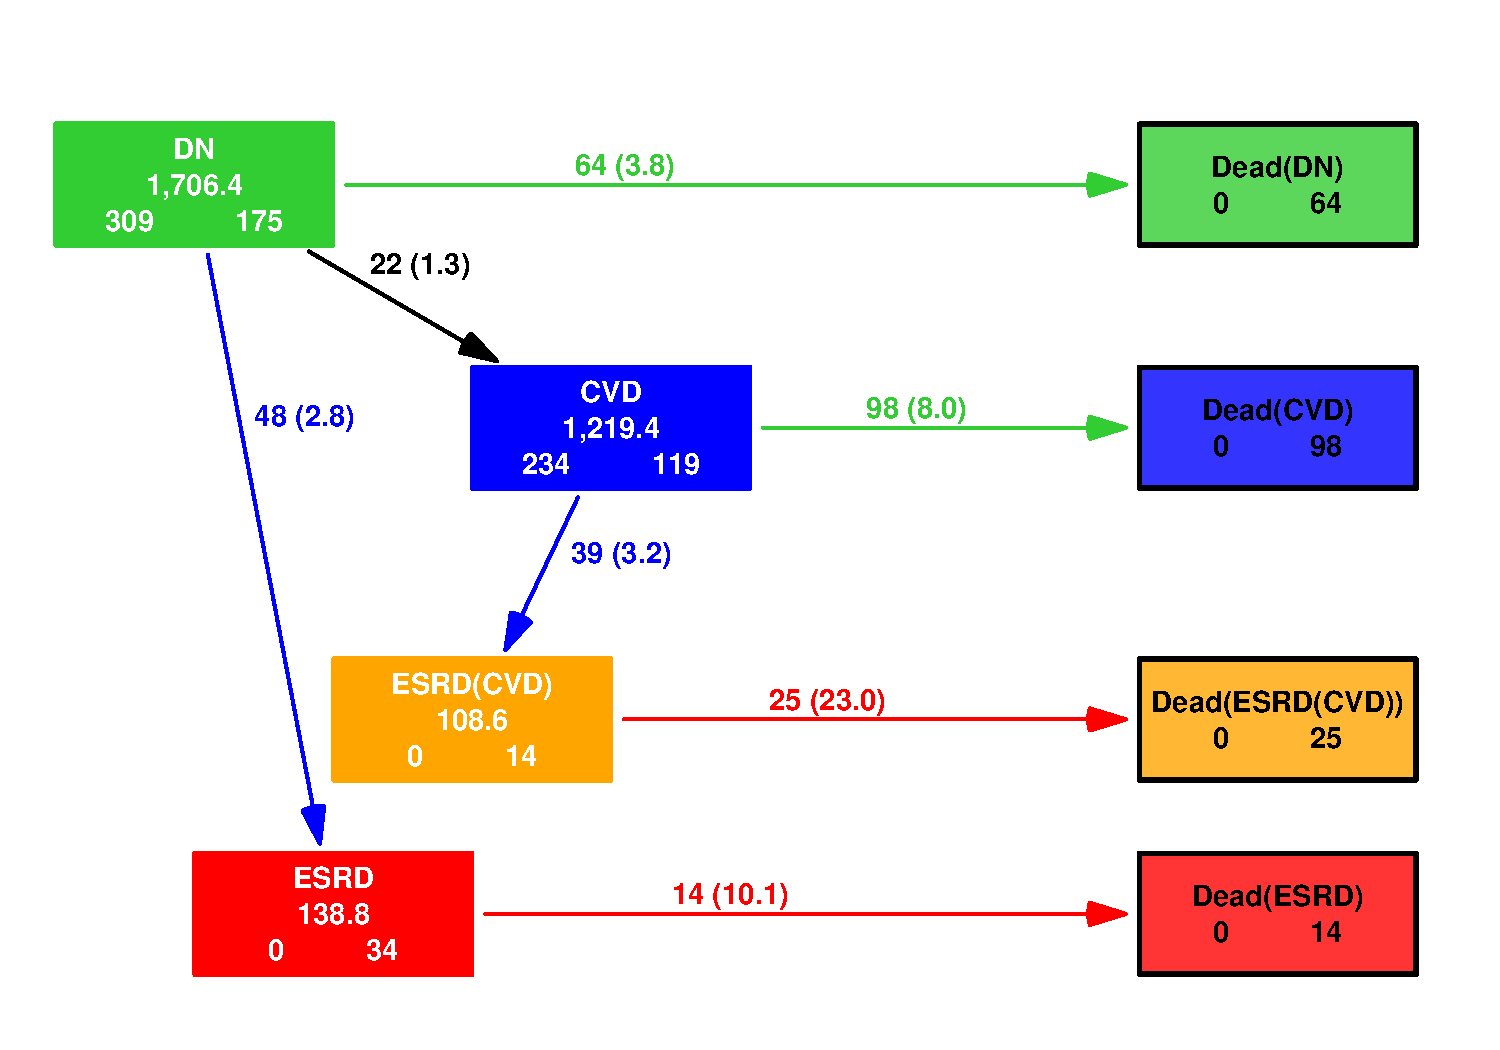
\includegraphics[width=0.82\textwidth]{./GbAd-states.pdf}
\end{frame}

%----------------------------------------------------------------------
\begin{frame}{A more complicated multistate model}
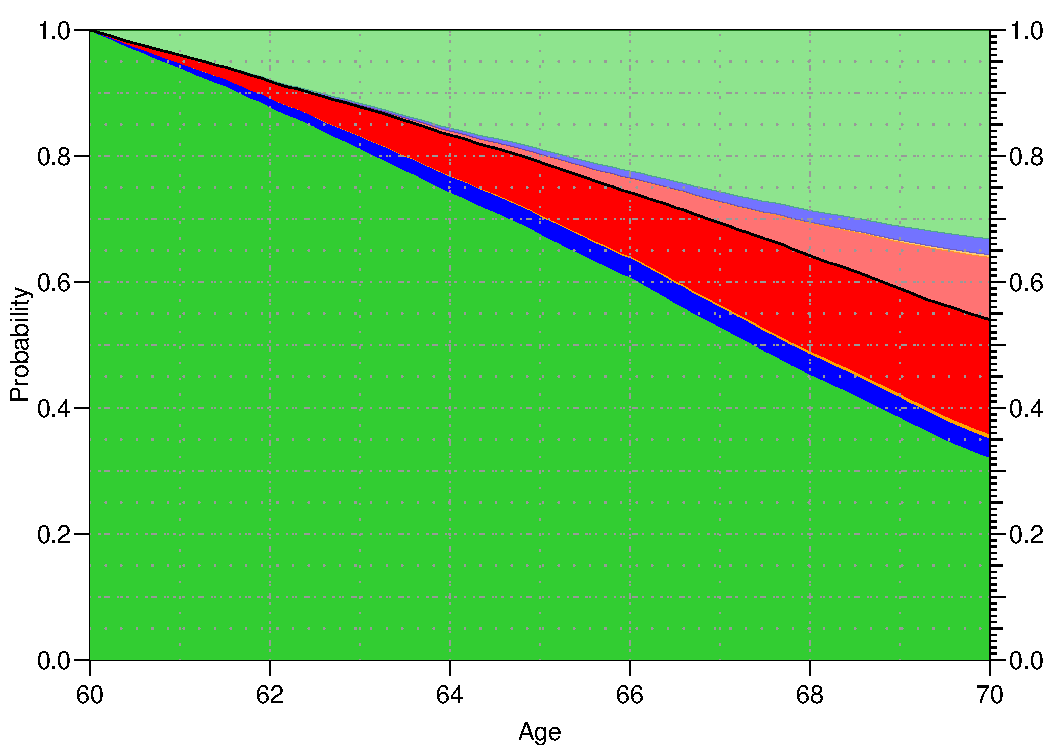
\includegraphics[width=0.75\textwidth]{./GbAd-probs.pdf}
\end{frame}
%----------------------------------------------------------------------


%----------------------------------------------------------------------
\begin{frame}
  \includegraphics[height=\textheight,keepaspectratio]{simRenal-states-col}
\end{frame}

%----------------------------------------------------------------------
\begin{frame}[fragile]{Modeling rates in a multistate model}
\pause
Each transition modeled by a model for rates\\ (Cox-model,
Poisson-model for split data, \texttt{glm} or \texttt{gam})

Requires that follow-up is split in small intervals:
\begin{Schunk}
\begin{Sinput}
> sLc <- splitLexis(Lc, "tfi", breaks = seq(0, 30, 1/12))
> summary(sLc)
\end{Sinput}
\begin{Soutput}
Transitions:
     To
From   NRA  Rem ESRD ESRD(Rem)  Records:  Events: Risk time:  Persons:
  NRA 9854   29   69         0      9952       98     824.77       122
  Rem    0 3139    0         8      3147        8     259.90        32
  Sum 9854 3168   69         8     13099      106    1084.67       125
\end{Soutput}
\end{Schunk}
\end{frame}

%----------------------------------------------------------------------
\begin{frame}[fragile]{Modeling rates in a multistate model}
\begin{Schunk}
\begin{Sinput}
> # Rem-rate
> mr <- gam(cbind(lex.Xst == "Rem", lex.dur)
+           ~ s(tfi, k = 10) + sex,
+           family = poisreg,
+             data = subset(sLc, lex.Cst == "NRA"))
> # ESRD-rates
> mx <- gam(cbind(lex.Xst %in% c("ESRD", "ESRD(Ren)"), lex.dur)
+           ~ s(tfi, k = 10) + sex + I((doe - dob - 40) / 10) + I(lex.Cst == "Rem"),
+           family = poisreg,
+             data = subset(sLc, lex.Cst %in% c("NRA", "Rem")))
\end{Sinput}
\end{Schunk}
\end{frame}

%----------------------------------------------------------------------
\begin{frame}[fragile]{\ldots using the \texttt{Lexis} properties}
\vspace*{-1em}
\begin{Schunk}
\begin{Sinput}
> # Remisson-rate
> mr <- gam.Lexis(sLc, from = "NRA", to = "Rem",
+                 formula = ~ s(tfi, k = 10) + sex)
\end{Sinput}
\begin{Soutput}
mgcv::gam Poisson analysis of Lexis object sLc with log link:
Rates for the transition:
NRA->Rem
\end{Soutput}
\begin{Sinput}
> # ESRD-rates
> mx <- gam.Lexis(sLc,
+                 formula = ~ s(tfi,k=10) + sex +
+                             I((doe - dob - 40) / 10) + I(lex.Cst == "Rem"))
\end{Sinput}
\begin{Soutput}
mgcv::gam Poisson analysis of Lexis object sLc with log link:
Rates for transitions:
NRA->ESRD
Rem->ESRD(Rem)
\end{Soutput}
\end{Schunk}
\vspace*{-1em}
Default is to model all transitions to absorbing states
\end{frame}

%----------------------------------------------------------------------
\begin{frame}{State probabilities}
   How do we get from rates (Poisson-models) to probabilities:
\pause
   \begin{itemize}[<+->]
   \item[1] Analytic calculations:

 \begin{itemize}[<+->]
     \item immensely complicated formulae
     \item computationally fast (once implemented)
     \item difficult to generalize
     \end{itemize}

   \item[2] Simulation of persons' histories

     \begin{itemize}[<+->]
     \item conceptually simple
     \item computationally not quite simple
     \item easy to generalize
     \item hard to get confidence intervals (bootstrap)
     \end{itemize}

   \end{itemize}
\end{frame}

%----------------------------------------------------------------------
\begin{frame}
   \frametitle{Simulation of a survival time}
   \begin{itemize}[<+->]
   \item For a rate function $\lambda(t)$,
     $\Lambda(t)=\int_0^t\lambda(s) \dif s$:
\[
   S(t) = \exp\bigl( -\Lambda(t) \bigr)
\]
   \item Simulate a survival probability $u \in [0,1]$:
\[
    u = S(t) \quad \Leftrightarrow \quad \Lambda(t) = -\log(u)
\]
   \item Knowledge of $\Lambda(t)$ makes it easy to find a survival time\\
      --- essentially just linear interpolation.
   \end{itemize}
\end{frame}

% %----------------------------------------------------------------------
% \begin{frame}[fragile]
%   \frametitle{Simulation of a survival time}
% Simulated random variate: $u$:
% \[
% u=0.853 \quad \Leftrightarrow \quad -\log(u) = 0.159
% \]
% Look up $0.159$ in the
% table of the cumulative rates $\Lambda(t)$:

% \renewcommand{\baselinestretch}{0.8}
% \small
% \begin{semiverbatim}
% time  Lambda
%  ...
%  1.2   0.131
%  1.3   \alert<2->{0.151}
%  1.4   \alert<2->{0.165}
%  1.5   0.181
%  ...
% \end{semiverbatim}
% \normalsize
% \renewcommand{\baselinestretch}{1.0}
% \pause
% \pause
% Linear interpolation gives:
% \[
% t = 1.3 + 0.1 \times (0.159-0.151)/(0.165-0.151) = 1.357
% \]
% \end{frame}

% %----------------------------------------------------------------------
% \begin{frame}
%    \frametitle{Simulation of one survival time}
%    \begin{itemize}[<+->]
%    \item Cumulative rates as a function of time
%    \item Obtained from a model for the mortality rates:

%      \begin{itemize}[<+->]
%      \item Cox-model:\\
%  Cumulative incidence directly --- the Breslow estimator
%      \item Poisson model:\\
%  Estimated incidence rates cumulated
%      \item \ldots
%      \end{itemize}
%    \item Simulate survival probability
%    \item Invert to time by look-up in table
%    \end{itemize}
% \end{frame}

%----------------------------------------------------------------------
\begin{frame}
   \frametitle{Simulation in a multistate model}
\vspace*{-1ex}
\includegraphics[width=0.45\textwidth]{simRenal-states-col}
\pause
\vspace*{-1ex}
   \begin{itemize}[<+->]
   \item Simulate a ``survival time'' for each transition
     \textbf{out} of a state.
   \item The smallest of these is the transition time.
   \item Choose the corresponding transition type as transition.
   \end{itemize}
\end{frame}

%----------------------------------------------------------------------
\begin{frame}[fragile]{Transition objects are \texttt{glm}/\texttt{gam}}
\vspace*{-1ex}
\includegraphics[width=0.45\textwidth]{simRenal-states-col}
\vspace*{-1ex}
\renewcommand{\baselinestretch}{0.8}
\small
\begin{Schunk}
\begin{Sinput}
> Tr <- list("NRA" = list("ESRD"      = mx,
+                         "Rem"       = mr),
+            "Rem" = list("ESRD(Rem)" = mx))
\end{Sinput}
\end{Schunk}
\normalsize
\renewcommand{\baselinestretch}{1.0}

\end{frame}

%----------------------------------------------------------------------
\begin{frame}{\texttt{simLexis}}
Input required:
   \begin{itemize}
   \item A \texttt{Lexis} object with the initial state of the
     persons to be simulated.\\
     (\texttt{lex.dur} and \texttt{lex.Xst} will be ignored---they are
     outcomes to be simulated)
 \item A transition object with the estimated Poisson models collected
   in a list of lists.
   \end{itemize}
\pause
Output produced:
\pause
\begin{itemize}
\item A \texttt{Lexis} object with simulated event histories for may
  persons
\end{itemize}

\end{frame}

%----------------------------------------------------------------------
\begin{frame}[fragile,allowframebreaks]{Using \texttt{simLexis}}
Put one record a new \texttt{Lexis} object (\texttt{init}, say).
representing a person with the desired covariate values.

Must have same structure as the one used for estimation --- time
scales must be initiated even if not used in models\\[-1ex]
\begin{Schunk}
\begin{Sinput}
> init <- sLc[NULL, c(timeScales(sLc), "lex.Cst")]
> init[1,"per"] <- 1994
> init[1,"age"] <- 40
> init[1,"tfi"] <- 0
> init[1,"lex.Cst"] <- "NRA"
> init[1,"sex"] <- "M"
> init[1,"dob"] <- 1954
> init[1,"doe"] <- 1994
> init
\end{Sinput}
\begin{Soutput}
  per age tfi lex.Cst sex  dob  doe
 1994  40   0     NRA   M 1954 1994
\end{Soutput}
\begin{Sinput}
> system.time(sim1 <- simLexis(Tr, init, N = 10000, t.range = 15))
\end{Sinput}
\begin{Soutput}
   user  system elapsed 
  24.69    1.52   26.21 
\end{Soutput}
\begin{Sinput}
> summary(sim1)
\end{Sinput}
\begin{Soutput}
Transitions:
     To
From  NRA  Rem ESRD ESRD(Rem)  Records:  Events: Risk time:  Persons:
  NRA 969 1847 7184         0     10000     9031   72599.26     10000
  Rem   0 1224    0       623      1847      623   15654.67      1847
  Sum 969 3071 7184       623     11847     9654   88253.94     10000
\end{Soutput}
\end{Schunk}
\pause
This is a simulated cohort of 10,000 persons with NRA aged 40 in 1994.
\end{frame}

%----------------------------------------------------------------------
\begin{frame}[fragile,allowframebreaks]{Using a simulated \texttt{Lexis} object --- \texttt{pState}}
\begin{Schunk}
\begin{Sinput}
> NN <- nState(sim1, at = seq(0, 15, 0.1),
+                  from = 0,
+            time.scale = "tfi")
> head(NN)
\end{Sinput}
\begin{Soutput}
     State
when    NRA   Rem  ESRD ESRD(Rem)
  0   10000     0     0         0
  0.1  9940    25    35         0
  0.2  9888    61    51         0
  0.3  9848    84    68         0
  0.4  9789   114    97         0
  0.5  9737   135   128         0
\end{Soutput}
\begin{Sinput}
> nw1 <- pState(NN, perm = c(1, 2, 4, 3))
> head(nw1, 3)
\end{Sinput}
\begin{Soutput}
     State
when     NRA    Rem ESRD(Rem) ESRD
  0   1.0000 1.0000    1.0000    1
  0.1 0.9940 0.9965    0.9965    1
  0.2 0.9888 0.9949    0.9949    1
\end{Soutput}
\begin{Sinput}
> tail(nw1, 3)
\end{Sinput}
\begin{Soutput}
      State
when      NRA        Rem ESRD(Rem) ESRD
  14.8 0.1020 0.22450000 0.2859000    1
  14.9 0.0992 0.22180000 0.2836000    1
  15   0.0000 0.06970925 0.1439466    1
\end{Soutput}
\begin{Sinput}
> par(mar = c(3, 3, 0.5, 2), mgp = c(3, 1, 0) / 1.6, las = 1)
> plot(nw1, col = clr[c(2, 1, 4, 3)] )
> lines(as.numeric(rownames(nw1)), nw1[,2], lwd = 2)
> axis(side = 4, at = 0:5 / 5)
> axis(side = 4, at = 0:10 / 10, labels = NA)
> axis(side = 4, at = 0:20 / 20, labels = NA, tcl = -0.3)
> axis(side = 4, at = 0:100/100, labels = NA, tcl = -0.2)
\end{Sinput}
\end{Schunk}
\begin{Schunk}
\begin{Sinput}
> nw2 <- pState( NN, perm = c(4,2,1,3) )
> head( nw2, 3 )
\end{Sinput}
\begin{Soutput}
     State
when  ESRD(Rem)    Rem    NRA ESRD
  0           0 0.0000 1.0000    1
  0.1         0 0.0025 0.9965    1
  0.2         0 0.0061 0.9949    1
\end{Soutput}
\begin{Sinput}
> tail( nw2, 3 )
\end{Sinput}
\begin{Soutput}
      State
when    ESRD(Rem)       Rem       NRA ESRD
  14.8 0.06140000 0.1839000 0.2859000    1
  14.9 0.06180000 0.1844000 0.2836000    1
  15   0.07423737 0.1439466 0.1439466    1
\end{Soutput}
\begin{Sinput}
> par(mar = c(3, 3, 0.5, 2), mgp = c(3, 1, 0) / 1.6, las = 1)
> plot(nw2, col = clr[c(4, 1, 2, 3)])
> axis(side = 4, at = 0:5 / 5)
> axis(side = 4, at = 0:10 / 10, labels = NA)
> axis(side = 4, at = 0:20 / 20, labels = NA, tcl = -0.3)
> axis(side = 4, at = 0:100/100, labels = NA, tcl = -0.2)
\end{Sinput}
\end{Schunk}
\end{frame}

%----------------------------------------------------------------------
\begin{frame}{Simulated probabilities}
\includegraphics[width=0.60\textwidth]{simRenal-nw1}
\end{frame}

%----------------------------------------------------------------------
\begin{frame}{Simulated probabilities}
\includegraphics[width=0.60\textwidth]{simRenal-nw2}
\end{frame}

%----------------------------------------------------------------------
\begin{frame}
   \frametitle{How many persons should you simulate?}
\pause
   \begin{itemize}[<+->]
   \item All probabilities have the same denominator --- the initial
     number of persons in the simulation, $N$, say.
   \item Thus, any probability will be of the form $p=x/N$
   \item For small probabilities we have that:
\[
 \se\bigl(\log(\hat p)\bigr) = (1-p)/\sqrt{N p (1-p)}
\]
\item So c.i. of the form $p\td \erf$ where:
\[
 \erf = \exp\bigl( 1.96 \times (1-p)/\sqrt{N p (1-p)} \bigr)
\]
   \end{itemize}
\end{frame}

%----------------------------------------------------------------------
\begin{frame}
   \frametitle{Precision of simulated probabilities}
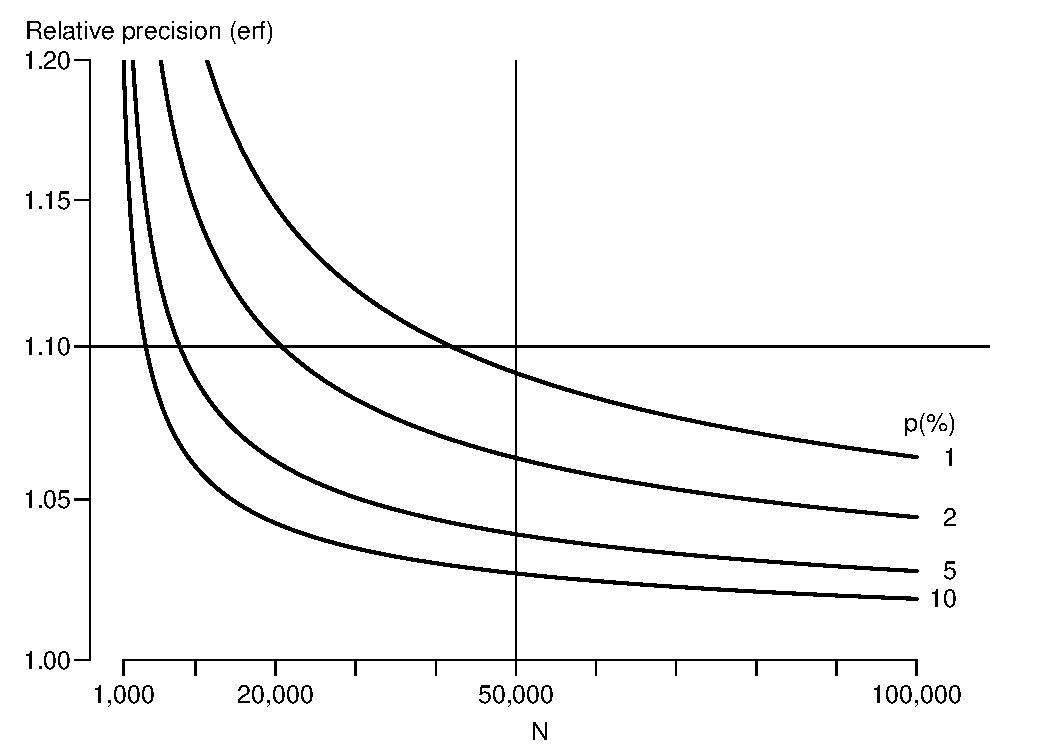
\includegraphics[width=0.75\textwidth]{./se-probs.pdf}
\end{frame}

%----------------------------------------------------------------------
\begin{frame}
   \frametitle{Multistate model overview}
\pause
   \begin{itemize}[<+->]
   \item Clarifies the relevant states and transitions are
   \item Allows proper estimation of transition rates
   \item --- and relationships between them
   \item Separate model for each transition
   \item The usual survival methodology to compute probabilities breaks down
   \item Simulation allows estimation of cumulative probabilities:

     \begin{itemize}[<+->]
     \item Estimate transition rates (as usual)
     \item Simulate probabilities (\textbf{not} quite as usual)
     \end{itemize}

   \end{itemize}
\end{frame}

\end{document}
